% This file is part of Combo Whist.
%
% Copyright 2007-2018 Joakim Nilsson
%
% This file is part of Combo Whist.
%
% Combo Whist is free software: you can redistribute it and/or modify
% it under the terms of the GNU General Public License as published by
% the Free Software Foundation, either version 3 of the License, or
% (at your option) any later version.
%
% Combo Whist is distributed in the hope that it will be useful,
% but WITHOUT ANY WARRANTY; without even the implied warranty of
% MERCHANTABILITY or FITNESS FOR A PARTICULAR PURPOSE.  See the
% GNU General Public License for more details.
%
% You should have received a copy of the GNU General Public License
% along with this text.  If not, see <http://www.gnu.org/licenses/>.

% Document class
\documentclass[a4paper]{article}

\usepackage[english]{babel}
% Packages
\usepackage[utf8]{inputenc}
\usepackage{graphicx}              % For \rotatebox
\usepackage{tabularx}              % For the X column specifier
\usepackage[pass]{geometry}        % For changing margins
\usepackage[labelfont=bf]{caption} % Captions boldface
\usepackage{verbatim}
\usepackage{hyperref}

% Set-up reference style
\hypersetup{%
	pdfborderstyle={/S/U/W 1}
}

% Rotate text 90 degrees
\newcommand{\rotccw}[1] {%
	\rotatebox{90}{{#1}}
}

\newcommand{\introPages}{%
	% Title
	\maketitle

	\vfill

	% Logo
	\begin{center}
		\includegraphics[width = \textwidth]{../logo.png}
	\end{center}

	\vfill

	% Copyright 2014-2024 Joakim Nilsson
%
% This file is part of Combo Whist.
%
% Combo Whist is free software: you can redistribute it and/or modify
% it under the terms of the GNU General Public License as published by
% the Free Software Foundation, either version 3 of the License, or
% (at your option) any later version.
%
% Combo Whist is distributed in the hope that it will be useful,
% but WITHOUT ANY WARRANTY; without even the implied warranty of
% MERCHANTABILITY or FITNESS FOR A PARTICULAR PURPOSE.  See the
% GNU General Public License for more details.
%
% You should have received a copy of the GNU General Public License
% along with Combo Whist.  If not, see <http://www.gnu.org/licenses/>.

% License notice
\begin{verbatim}
	Copyright 2007-2024 Joakim Nilsson

	This document is part of Combo Whist.

	Combo Whist is free software: you can redistribute it and/or modify
	it under the terms of the GNU General Public License as published by
	the Free Software Foundation, either version 3 of the License, or
	(at your option) any later version.

	Combo Whist is distributed in the hope that it will be useful,
	but WITHOUT ANY WARRANTY; without even the implied warranty of
	MERCHANTABILITY or FITNESS FOR A PARTICULAR PURPOSE.  See the
	GNU General Public License for more details.
\end{verbatim}
\verb|You should have received a copy of the GNU General Public License|\\
\verb|along with Combo Whist.  If not, see <|\url{http://www.gnu.org/licenses/}\verb|>.|


	\thispagestyle{empty}
	\pagebreak

	% Table of contents and list of tables
	\setcounter{tocdepth}{3}
	\tableofcontents
	\listoftables
	\thispagestyle{empty}
	\pagebreak
}


% Title
\title{Combo Whist}
\author{By Joakim Nilsson}
\ifdefined\varDev
	\date{Development version (based on version \varVersion-\varLanguage) --- \today}
\else
	\date{Version \varVersion-\varLanguage\ --- \today}
\fi

% Document
\begin{document}
	\introPages

	\section{Overview}
		Combo Whist is a trick-taking card game and, as its name implies, is a variant of Whist. The key trait of Combo Whist is its great variety of available strategies while still having a rule set that is fairly simple (although the rule set is undeniably somewhat large). The many and varied strategies avoids a substantial amount of randomness that is usually present in Whist games without making the game overly complicated, keeping it fun to play for both experienced and casual card players.

		\paragraph{Number of players:}
			Preferably 4, but 3 to $\infty$ is also possible with some modifications to the rules.

		\paragraph{Requirements:}
			A standard 52 card deck, a pen and a piece of paper.

		\paragraph{Card rank:}
			From highest to lowest: A, K, Q, J, 10, 9, 8, 7, 6, 5, 4, 3, 2

	\section{How to play}
		\subsection{Preparations}
			On the paper, make a column for each player. This is for keeping track of each players' score as well as some other information about the game. After you have properly prepared the paper, choose a dealer at random.

			If there are only 3 players, $\spadesuit 6$, as well as all the 9s, 8s and 7s are removed from the deck.

		\subsection{Deal}
			There are two main parts of a deal. The first part is the \emph{bidding} and the second part is the \emph{game}. As things should be easier to understand in the reverse order, we will describe the game before the bidding.

			A deal begins by the dealer dealing 13 cards to each player. Next, the bidding begins and when it has finished, the game begins.

			After the game, players' new scores are noted down and a new deal begins with the next dealer being the player who is seated to the left of the current dealer.

			\subsubsection{Game}
				The game plays similarly to any Whist variant. The player to the right of the \emph{declarer}\footnote{The term ``declarer'' is explained in the \textit{\nameref{sec:bidding}} section.} begins by playing a card. Next, the player to the left of them plays a card which must follow the suit of the first card. After that, the next player (one step further left) plays yet another card which must also follow the suit of the first card, and so on until all players have played one card each.

				If a player is out of cards in the leading suit, they may discard any card or play a trump. Unlike many variants of Whist, there is no obligation to play a trump when you are out of cards in the leading suit.

				The player who played the highest card in the leading suit takes the \emph{trick} (that is, takes all the played cards and puts them face down on the table) unless a trump is played, in which case the player who played the highest trump takes the trick. The player who brought home the last trick leads the next one.

			\subsubsection{Bidding}
				\label{sec:bidding}
				In Combo Whist, players make \emph{combo bids}. A combo bid is composed of exactly one standard bid and any amount (including zero) of unique special bids. The bids have rules associated with them that are applied during the game and during scoring. If it is unclear \emph{when} an event triggered by a bid is supposed to occur, the standard bids take priority before the special bids.

				The players take turns by bidding in a clockwise manner and the player to the left of the dealer makes the first bid. A player can either pass or make a combo bid that is worth more than the previous combo bid (from here on simply referred to as a \emph{bid}). If a player passes, they are out of the bidding and may therefore not make any new bids until the next deal. If all players pass, the same dealer collects all cards and deals a new deal.

				A bid's worth is defined as the combined worth of the standard and special bids it comprises. A proposed time limit between each bid is 20 seconds and 1 minute before the initial bid, but for beginners higher limits or no limits are recommended. If a player hasn't made a bid within the given time limit, they automatically pass. The bidding continues until all players but one have passed. That player becomes declarer and the game begins.

				The available standard and special bids are listed in Tables~\ref{tab:standardBids}~and~\ref{tab:specialBids}, respectively. The number of tricks to bring home to complete the bid is given in the standard bids table in the ``Tricks'' column. A special bid cannot be combined with another bid listed in the ``Incompatibility'' column, nor are combo bids allowed which are impossible to complete regardless of the distribution of cards. Note that there is a difference between worth and score. Worth is the bid's worth (You guessed it!) and score is the number of points the declarer scores if they complete the bid.
			

			\subsubsection{Scoring}
				After the game has finished the declarer scores a number of points determined by what combo bid was bid and whether it was completed. If the bid was completed, they score as many points as as noted in the ``Score'' column for the standard bid. If the bid was not completed, 2 points are subtracted from their previous score count. It is possible to attain a negative score. If a player has a score below $-5$, they are not allowed to bid during bidding. However, they automatically gain 1 point when that deal is completed (even if no one bids).

			\subsubsection{Winning}
				The winner is the player who first scores the \emph{winning score}. The winning score starts at 13, but 1 is subtracted from it every time all players have dealt one deal each until the winning score reaches 1. A player must win by completing a bid and can therefore not win solely because the winning score just decreased. A player can also not win unless they have the highest score alone. If all players but one attains a score of $-5$, the player who has the higher score automatically wins, regardless of the winning score. This type of win is called \emph{a Win of Shame}.

	\section{Miscellaneous}
		\subsection{Rules for more than 4 players}
			If there are more than 4 players participating in the game, for every deal, all players but 4 sits out (that is, they don't participate in the deal). These players are the ones that are closest to the right of the dealer.
		
		\subsection{Talking}
			A certain amount of talk is allowed in Combo Whist, but the players are not allowed to give \emph{any} hints about what cards they have.
		
		\subsection{Cheating}
			A player who intentionally cheats in Combo Whist is never again allowed to play it because it is obvious that they don't respect the game's magnificence.

	% Bid tables
	\pagebreak
	\newgeometry{left=1cm, right=1cm, top=1cm}
	% Copyright 2007-2021 Joakim Nilsson
%
% This file is part of Combo Whist.
%
% Combo Whist is free software: you can redistribute it and/or modify
% it under the terms of the GNU General Public License as published by
% the Free Software Foundation, either version 3 of the License, or
% (at your option) any later version.
%
% Combo Whist is distributed in the hope that it will be useful,
% but WITHOUT ANY WARRANTY; without even the implied warranty of
% MERCHANTABILITY or FITNESS FOR A PARTICULAR PURPOSE.  See the
% GNU General Public License for more details.
%
% You should have received a copy of the GNU General Public License
% along with Combo Whist.  If not, see <http://www.gnu.org/licenses/>.

\section{Standardbud}
	\begin{center}
		\begin{tabularx}{\textwidth}{
			l
			S[table-number-alignment=center, table-format=1.0]
			S[table-number-alignment=center, table-format=1.0]
			cc|X
		}
				\textbf{Benämning} &
				\rotccw{\textbf{Värde}} &
				\rotccw{\textbf{Poäng}} &
				\rotccw{\textbf{Trumf}} &
				\rotccw{\textbf{Stick}} &
				\textbf{Tilläggsregler}
				\\[-3ex]

				\standardBidItem%
				{Skambud}
				{0}
				{1}
				{nej}
				{varierar}
				{%
					Spelföraren får inte ta hem flest stick---inte ens om nån annan spelare har tagit hem lika många stick.
				}

				\standardBidItem%
				{Trumf}
				{1}
				{1}
				{ja}
				{min 5}
				{%
					Spelföraren bestämmer trumffärg.
				}

				\standardBidItem%
				{Ungefär}
				{1}
				{1}
				{nej}
				{varierar}
				{%
					Före spelets början gissar spelföraren på två möjliga mängder stick denne kommer att ta hem. Spelföraren måste ta hem en av de möjliga mängderna stick som gissades.
				}

				\standardBidItem%
				{Grill}
				{1}
				{2}
				{ja}
				{min 5}
				{%
					Spelföraren börjar med att bestämma trumffärg. Denna trumffärg gäller bara första sticket. Därefter blir den färg som spelades ut i föregångde stick ny trumffärg och så fortsätter det till spelets slut.
				}

				\standardBidItem%
				{Blocktrumf}
				{2}
				{1}
				{ja}
				{min 5}
				{%
					Spelföraren bestämmer trumffärg. Spelföraren får inte spela något trumfkort förrän någon annan splare spelar trumf (såvida inte spelföraren enbart besitter trumfkort).
				}
				
				\standardBidItem%
				{Limbo}
				{2}
				{1}
				{nej}
				{varierar}
				{%
					Spelföraren måste ta hem färre stick av de 7 första sticken än av de 6 sista.
				}
				
				\standardBidItem%
				{Spel}
				{2}
				{2}
				{nej}
				{min 5}
				{%
					---
				}

				\standardBidItem%
				{Exakt}
				{3}
				{2}
				{nej}
				{varierar}
				{%
					Före spelets början gissar spelföraren på en möjlig mängd stick denne kommer att ta hem. Spelföraren måste ta hem den mängd stick som gissades.
				}

				\standardBidItem%
				{Mästarskambud}
				{3}
				{2}
				{nej}
				{varierar}
				{%
					Spelföraren måste ta hem färst stick. Om ingen tar hem färre stick än spelföraren går budet hem.
				}

				\standardBidItem%
				{Maxtrumf}
				{3}
				{3}
				{ja}
				{min 7}
				{%
					Spelföraren väljer trumffärg.
				}

				\standardBidItem%
				{Subtrumf}
				{3}
				{3}
				{ja}
				{min 5}
				{%
					Spelföraren väljer trumffärg. Denne får dock inte välja en trumffärg som denne har flest kort i.
				}

				\standardBidItem%
				{Rangtrumf}
				{3}
				{4}
				{ja}
				{min 5}
				{%
					Alla spelare väljer ett kort var och lägger det på bordet med bildsidan nedåt. Korten vänds sedan upp och spelföraren byter ut sitt kort med det av motspelarnas som är högst. Skulle det finnas flera högsta kort väljer spelföraren ett av dem. Det valda kortets färg är trumffärgen.
				}

				\standardBidItem%
				{Mästarspel}
				{4}
				{3}
				{nej}
				{varierar}
				{%
					Spelföraren måste ta hem enskilt flest stick.
				}

				\standardBidItem%
				{Noll}
				{4}
				{4}
				{nej}
				{0}
				{%
					---
				}

				\standardBidItem%
				{Mästartrumf}
				{6}
				{6}
				{ja}
				{min 5}
				{%
					Spelaren till vänster om spelföraren bestämmer trumffärg, men först får de andra icke-spelförarna säga vilken trumffärg de föredrar och hur mycket de föredrar denna på en skala från 1 till 5 (utan motivering).
				}

				\standardBidItem%
				{Obesudlat Mästarspel}
				{9}
				{*}
				{nej}
				{13}
				{%
					*Om budet går hem får spelföraren lika många poäng som kombinationsbudets värde. Skulle dessutom kombinationsbudets värde vara 13 eller högre vinner spelföraren spelet omedelbart, oavsett poängställning. När detta inträffar erhåller dessutom spelföraren rätten att titulera sig \emph{Obesudlad~Mästare~av~Kombinations-Whist} under resten av sitt liv.
				}
		\end{tabularx}
	\end{center}

	% This file is part of Combo Whist.
%
% Copyright 2007-2019 Joakim Nilsson
%
% This file is part of Combo Whist.
%
% Combo Whist is free software: you can redistribute it and/or modify
% it under the terms of the GNU General Public License as published by
% the Free Software Foundation, either version 3 of the License, or
% (at your option) any later version.
%
% Combo Whist is distributed in the hope that it will be useful,
% but WITHOUT ANY WARRANTY; without even the implied warranty of
% MERCHANTABILITY or FITNESS FOR A PARTICULAR PURPOSE.  See the
% GNU General Public License for more details.
%
% You should have received a copy of the GNU General Public License
% along with this text.  If not, see <http://www.gnu.org/licenses/>.

\newcommand{\nonTrump}{\textnormal{non-trump bids}}

\begin{table}
	\caption{Special bids}\label{tab:specialBids}
	\begin{center}
		\begin{tabularx}{\textwidth}{
			l
			S[table-number-alignment=center, table-figures-decimal=0]
			p{3cm}
			|X
		}
			\textbf{Name} &
			\textbf{Worth} &
			\textbf{Incompatibility} &
			\textbf{Additional rules}
			\\[-3ex]

			\specialBidItem%
			{Triumph Trump}
			{-4}
			{---}
			{%
				The declarer selects any card before the game begins. This card becomes the \emph{triumph trump}. The declarer decides who takes a trick containing the triumph trump when this trick is brought home. A triumph trump does \emph{not} change suit to the trumph suit, but retains its old suit.
			}

			\specialBidItem%
			{Sloth}
			{-3}
			{---}
			{%
				For the tricks in which the declarer doesn't lead, the declarer plays last.
			}

			\specialBidItem%
			{Potential}
			{-2}
			{---}
			{%
				If this bid is completed it is marked by a P, a \emph{potential}, in the declarer's column. The worth of all the declarer's future combo bids increase by \sfrac{1}{2} for each P in the declarer's column.
			}

			\specialBidItem%
			{Start}
			{-2}
			{---}
			{%
				The declarer leads the first trick.
			}

			\specialBidItem%
			{Iron}
			{-1}
			{---}
			{%
				The aces now rank the lowest.
			}

			\specialBidItem%
			{Switcheroo}
			{-1}
			{---}
			{%
				Before the game starts, all players send 3 cards in a direction the declarer chooses (to the right, to the left or across).
			}

			\specialBidItem%
			{Greed}
			{0}
			{---}
			{%
				At the end of the game, one virtual trick is added to or subtracted from the declarer's stick count in such a way that it disfavors them. If the bid is completed, the declarer scores 1 extra point.
			}

			\specialBidItem%
			{Atelier}
			{1}
			{Open~Hand}
			{%
				The declarer chooses 4 cards that they put in \emph{the atelier}. These cards must be shown to all players during the game. As soon as the atelier no longer consists of 4 cards, the declarer must add a card to it, if possible.
			}

			\specialBidItem%
			{Ending Dog}
			{1}
			{Zero}
			{%
				The declarer must not bring home the last trick.
			}

			\specialBidItem%
			{Open Trump}
			{1}
			{\nonTrump, Grill, Open~Hand}
			{%
				The declarer must play with open trump cards. That is, all of the declarer’s trump cards must be shown to all players during the game. If combined with \emph{Atelier}, the atelier must not contain any trump cards.
			}

			\specialBidItem%
			{Lock}
			{2}
			{Zero}
			{%
				The declarer must not bring home any of the first 3 tricks.
			}

			\specialBidItem%
			{Plague}
			{2}
			{Bid~of~Shame, Master's~Bid~of~Shame, Zero}
			{%
				The declarer chooses a suit to be the \emph{plague suit}. The declarer must not become \emph{beplagued}; That is, must not alone bring home the most plague cards (note: \emph{not} tricks), unless they become \emph{honourbly beplagued} and bring home the whole plague suit, in which case they also score an honourable extra point.
			}

			\specialBidItem%
			{Penalty}
			{2}
			{---}
			{%
				If the declarer does not complete their bid, 2 extra points are subtracted from their score.
			}

			\specialBidItem%
			{Master's Switcheroo}
			{3}
			{\nonTrump, Grill}
			{%
				Before the game starts, all players but the declarer sends 4 cards to the player to the right (skipping the declarer). If \emph{Switcheroo} has been bid, the \emph{Switcheroo}-cards are sent before the \emph{Master's Switcheroo}-cards.
			}

			\specialBidItem%
			{Open Hand}
			{3}
			{Atelier, Open~Trump}
			{%
				The declarer must play with an open hand. That is, all of the their cards must be shown to all players during the game.
			}
		\end{tabularx}
	\end{center}
\end{table}

\end{document}
